% Provenance (never printed): see sources/outline_sources.md and sources/book1/BRIEFS.md (g9/02).
\chapter{Logic Gates and Boolean Algebra}\label{ch:g9:logic-gates}

A lift moves only if its door is closed \emph{and} a floor button has been
pressed. A hall light comes on if this switch \emph{or} the one at the other
end of the hall is on. Inside a \omterm{def:g1:what-is-a-computer:computer}{computer}, billions of tiny parts make such
decisions on \omterm{def:g5:bits-and-bytes:bit}{bits}, billions of times a second. This chapter builds them, from
the smallest one to a circuit that adds.

\begin{recall}
A \omterm{def:g6:if-else:comparison}{Boolean value} is \code{True} or \code{False}; \code{and}, \code{or} and
\code{not} combine them, and a table of the four cases shows the result of
\code{and} and \code{or} (\cref{ch:g6:if-else}). Two \omterm{def:g5:bits-and-bytes:bit}{bits} are added column by
column, with a \omterm{def:g8:binary-and-hexadecimal:carry}{carry}; $n$ \omterm{def:g5:bits-and-bytes:bit}{bits} make $2^n$ patterns
(\cref{ch:g8:binary-and-hexadecimal}).
\end{recall}

\section{True and false as 1 and 0}

A \omterm{def:g5:bits-and-bytes:bit}{bit} has two \omterm{def:g6:variables-and-input:value}{values}, like a \omterm{def:g6:if-else:comparison}{Boolean value}: 1 can stand for true and 0 for
false. Python itself counts \code{True} as 1 and \code{False} as 0:

\Needspace*{5\baselineskip}
\omcode{code/grade-9/02-logic-gates/listings/bits.py}{1}{2}{Booleans are
numbers.}\label{lst:g9:logic-gates:bits}

\Needspace*{6\baselineskip}
\omoutput{code/grade-9/02-logic-gates/outputs/bits.txt}{\code{True + True} is
2.}\label{out:g9:logic-gates:bits}

In this chapter, every \omterm{def:g6:variables-and-input:value}{value} is a \omterm{def:g5:bits-and-bytes:bit}{bit}, 0 or 1, and the operations are written
in capitals, NOT, AND, OR, to keep them apart from Python's words.

\section{Gates and their truth tables}

\begin{definition}[Logic gate, truth table]\label{def:g9:logic-gates:gate}\label{def:g9:logic-gates:truth-table}
A \emph{logic gate}\index{logic gate} is a small circuit that takes one or two
\omterm{def:g5:bits-and-bytes:bit}{bits} as \omterm{def:g1:what-is-a-computer:input}{inputs} and gives one \omterm{def:g5:bits-and-bytes:bit}{bit} as \omterm{def:g1:what-is-a-computer:input}{output}. Its \emph{truth
table}\index{truth table} \omterm{def:g7:lists:list}{lists} the \omterm{def:g1:what-is-a-computer:input}{output} for every possible \omterm{def:g1:what-is-a-computer:input}{input}.
\end{definition}

\begin{definition}[NOT, AND, OR and XOR gates]\label{def:g9:logic-gates:not-and-or-xor}
The \emph{NOT gate}\index{NOT gate} gives 1 when its \omterm{def:g1:what-is-a-computer:input}{input} is 0, and 0 when it
is 1. The \emph{AND gate}\index{AND gate} gives 1 only when both \omterm{def:g1:what-is-a-computer:input}{inputs} are 1.
The \emph{OR gate}\index{OR gate} gives 1 when at least one \omterm{def:g1:what-is-a-computer:input}{input} is 1. The
\emph{XOR gate}\index{XOR gate} (for \emph{exclusive or}) gives 1 when exactly
one \omterm{def:g1:what-is-a-computer:input}{input} is 1.
\end{definition}

With \omterm{def:g5:bits-and-bytes:bit}{bits}, each gate is a little arithmetic: AND is a product, NOT is $1 - a$,
XOR is the remainder of $a + b$ divided by 2.

\omcode{code/grade-9/02-logic-gates/listings/gates.py}{1}{22}{The four gates as
\omterm{def:g7:functions:function}{functions}, and their tables.}\label{lst:g9:logic-gates:gates}

\Needspace*{10\baselineskip}
\omoutput{code/grade-9/02-logic-gates/outputs/gates.txt}{The \omterm{def:g9:logic-gates:gate}{truth tables} of the
four gates.}\label{out:g9:logic-gates:gates}

\begin{omfigure}
\begin{circuitikz}[font=\small]
  \node[not port] (N) at (1.5,0) {};
  \draw (N.in) -- ++(-0.5,0) node[left] {$a$};
  \draw (N.out) -- ++(0.4,0) node[right] {out};
  \node[anchor=south, font=\small\bfseries] at (1.5,0.5) {NOT};
  \node[anchor=west, font=\scriptsize\ttfamily, align=left] at (3.4,0) {a | out\\ 0 | 1\\ 1 | 0};
  \foreach \kind/\name/\x/\y/\rows in {and port/AND/7.5/0/{0 0 | 0\\ 0 1 | 0\\ 1 0 | 0\\ 1 1 | 1}, or port/OR/1.5/-3.0/{0 0 | 0\\ 0 1 | 1\\ 1 0 | 1\\ 1 1 | 1}, xor port/XOR/7.5/-3.0/{0 0 | 0\\ 0 1 | 1\\ 1 0 | 1\\ 1 1 | 0}} {
    \node[\kind] (g) at (\x,\y) {};
    \draw (g.in 1) -- ++(-0.5,0) node[left] {$a$};
    \draw (g.in 2) -- ++(-0.5,0) node[left] {$b$};
    \draw (g.out) -- ++(0.4,0) node[right] {out};
    \node[anchor=south, font=\small\bfseries] at (\x,\y+0.5) {\name};
    \node[anchor=west, font=\scriptsize\ttfamily, align=left] at (\x+1.9,\y) {a b | out\\ \rows};
  }
\end{circuitikz}

{\small The symbols of the NOT, AND, OR and \omterm{def:g9:logic-gates:not-and-or-xor}{XOR gates}, each with its \omterm{def:g9:logic-gates:gate}{truth
table}. The \omterm{def:g1:what-is-a-computer:input}{inputs} come in on the left, the \omterm{def:g1:what-is-a-computer:input}{output} leaves on the right; NOT's
small circle means ``the opposite''.}
\end{omfigure}

\section{Circuits of gates}

\begin{definition}[Logic circuit]\label{def:g9:logic-gates:circuit}
A \emph{logic circuit}\index{logic circuit} is a set of gates wired together,
the \omterm{def:g1:what-is-a-computer:input}{output} of one gate feeding an \omterm{def:g1:what-is-a-computer:input}{input} of another. Its \omterm{def:g9:logic-gates:gate}{truth table} gives its
\omterm{def:g1:what-is-a-computer:input}{output} for each of the $2^n$ patterns of its $n$ \omterm{def:g1:what-is-a-computer:input}{inputs}.
\end{definition}

The circuit below computes \code{(a AND b) OR (NOT c)}. Three \omterm{def:g1:what-is-a-computer:input}{inputs} make
$2^3 = 8$ rows, and three \omterm{def:g6:for-loops-turtle:nested}{nested loops} go through them in the order of
counting in \omterm{def:g5:bits-and-bytes:binary}{binary}, from \code{0 0 0} to \code{1 1 1}:

\omcode{code/grade-9/02-logic-gates/listings/circuit.py}{1}{13}{The \omterm{def:g9:logic-gates:gate}{truth table} of
a circuit with three \omterm{def:g1:what-is-a-computer:input}{inputs}.}\label{lst:g9:logic-gates:circuit}

\Needspace*{13\baselineskip}
\omoutput{code/grade-9/02-logic-gates/outputs/circuit.txt}{8 rows, one per
pattern of three \omterm{def:g5:bits-and-bytes:bit}{bits}.}\label{out:g9:logic-gates:circuit}

\begin{omfigure}
\begin{circuitikz}[font=\small]
  \node[and port] (A) at (2.5,0.6) {};
  \node[not port] (N) at (2.3,-0.9) {};
  \node[or port] (O) at (5.0,-0.1) {};
  \draw (0,0 |- A.in 1) node[left] {$a$} -- (A.in 1);
  \draw (0,0 |- A.in 2) node[left] {$b$} -- (A.in 2);
  \draw (0,-0.9) node[left] {$c$} -- (N.in);
  \draw (A.out) -| ($(O.in 1)+(-0.4,0)$) -- (O.in 1);
  \draw (N.out) -| ($(O.in 2)+(-0.4,0)$) -- (O.in 2);
  \draw (O.out) -- ++(0.5,0) node[right] {out};
\end{circuitikz}

{\small The circuit \code{(a AND b) OR (NOT c)}: two gates feed a third. Its
table is the \omterm{def:g1:what-is-a-computer:input}{output} of \cref{lst:g9:logic-gates:circuit}.}
\end{omfigure}

Two different circuits can compute the same thing. To be sure, compare them on
every \omterm{def:g1:what-is-a-computer:input}{input}: with two \omterm{def:g1:what-is-a-computer:input}{inputs} there are only four.

\omcode{code/grade-9/02-logic-gates/listings/same_circuit.py}{1}{18}{Two circuits
compared on every \omterm{def:g1:what-is-a-computer:input}{input}.}\label{lst:g9:logic-gates:same}

\Needspace*{9\baselineskip}
\omoutput{code/grade-9/02-logic-gates/outputs/same_circuit.txt}{Always the same
\omterm{def:g1:what-is-a-computer:input}{output}.}\label{out:g9:logic-gates:same}

\section{Rules of Boolean algebra}

% ledger: g9:boole-1854
In 1854, the English mathematician George Boole published a book that treated
reasoning as a kind of algebra, with letters for true and false statements.
The rules of that algebra, now called Boolean, hold for gates:

\begin{center}\small
\begin{tabular}{@{}ll@{}}
NOT (NOT $a$) $= a$ & \\
$a$ AND 1 $= a$ & $a$ OR 0 $= a$ \\
$a$ AND 0 $= 0$ & $a$ OR 1 $= 1$ \\
$a$ AND $a = a$ & $a$ OR $a = a$ \\
$a$ AND (NOT $a$) $= 0$ & $a$ OR (NOT $a$) $= 1$ \\
\end{tabular}
\end{center}

Each rule is checked by trying both \omterm{def:g6:variables-and-input:value}{values} of $a$. For instance,
$a$ OR 1: if $a = 0$, then $0$ OR $1 = 1$; if $a = 1$, then $1$ OR $1 = 1$.

\begin{proposition}[De Morgan's laws for gates]\label{prop:g9:logic-gates:de-morgan}
For any \omterm{def:g5:bits-and-bytes:bit}{bits} $a$ and $b$,
NOT ($a$ AND $b$) $=$ (NOT $a$) OR (NOT $b$), and
NOT ($a$ OR $b$) $=$ (NOT $a$) AND (NOT $b$).
\index{De Morgan's laws (for gates)}
\end{proposition}

\begin{proof}
Two \omterm{def:g5:bits-and-bytes:bit}{bits} have only four patterns. The \omterm{def:g4:programs-and-operating-system:program}{program} below computes both sides of
each law for all four, and the two columns of each law are equal on every row.
\end{proof}

\Needspace*{11\baselineskip}
\omcode{code/grade-9/02-logic-gates/listings/de_morgan.py}{1}{8}{Both sides of De
Morgan's laws.}\label{lst:g9:logic-gates:de-morgan}

\Needspace*{9\baselineskip}
\omoutput{code/grade-9/02-logic-gates/outputs/de_morgan.txt}{Equal columns, row
by row.}\label{out:g9:logic-gates:de-morgan}

In words: ``not both'' is ``one of them is not'', and ``neither'' is ``this
one is not, and that one is not''. The circuits of
\cref{lst:g9:logic-gates:same} were the first law.

\section{The half adder; the transistor as a switch}

\begin{definition}[Half adder]\label{def:g9:logic-gates:half-adder}
A \emph{half adder}\index{half adder} is a circuit that adds two \omterm{def:g5:bits-and-bytes:bit}{bits}. It has
two \omterm{def:g1:what-is-a-computer:input}{outputs}: the \emph{sum} \omterm{def:g5:bits-and-bytes:bit}{bit}, $a$ XOR $b$, and the \emph{\omterm{def:g8:binary-and-hexadecimal:carry}{carry}} \omterm{def:g5:bits-and-bytes:bit}{bit}, $a$
AND $b$.
\end{definition}

$1 + 1 = 2$, written \code{10} in \omterm{def:g5:bits-and-bytes:binary}{binary}: a sum \omterm{def:g5:bits-and-bytes:bit}{bit} 0 and a \omterm{def:g8:binary-and-hexadecimal:carry}{carry} 1, as in the
column additions of \cref{ch:g8:binary-and-hexadecimal}.

\omcode{code/grade-9/02-logic-gates/listings/half_adder.py}{1}{13}{The \omterm{def:g9:logic-gates:half-adder}{half adder}:
two gates.}\label{lst:g9:logic-gates:half-adder}

\Needspace*{9\baselineskip}
\omoutput{code/grade-9/02-logic-gates/outputs/half_adder.txt}{The four sums of two
\omterm{def:g5:bits-and-bytes:bit}{bits}.}\label{out:g9:logic-gates:half-adder}

The \omterm{def:g7:functions:function}{function} returns two \omterm{def:g6:variables-and-input:value}{values}; \code{total, carry = half_adder(a, b)} puts
the first in \code{total} and the second in \code{carry}.

\begin{omfigure}
\begin{circuitikz}[font=\small, dot/.style={circle, fill, inner sep=0pt, minimum size=3pt}]
  \node[xor port] (X) at (3,0.8) {};
  \node[and port] (A) at (3,-0.8) {};
  \draw (0,0 |- X.in 1) node[left] {$a$} -- (X.in 1);
  \draw (0,0 |- X.in 2) node[left] {$b$} -- (X.in 2);
  \draw (0.6,0 |- X.in 1) node[dot] {} |- (A.in 1);
  \draw (1.1,0 |- X.in 2) node[dot] {} |- (A.in 2);
  \draw (X.out) -- ++(0.5,0) node[right] {sum};
  \draw (A.out) -- ++(0.5,0) node[right] {carry};
\end{circuitikz}

{\small The \omterm{def:g9:logic-gates:half-adder}{half adder}: an \omterm{def:g9:logic-gates:not-and-or-xor}{XOR gate} and an \omterm{def:g9:logic-gates:not-and-or-xor}{AND gate} share the same two
\omterm{def:g1:what-is-a-computer:input}{inputs}.}
\end{omfigure}

Every addition a \omterm{def:g1:what-is-a-computer:computer}{computer} makes is built from such circuits, chained column
after column; the next book builds them. And what is a gate made of? Of
\emph{transistors}: tiny switches that are opened and closed by electricity
instead of a finger. The physics books explain electric circuits and their
switches; here, only one fact matters. Two switches in a row, in
\emph{series}, let the current through only if both are closed: AND. Two
switches side by side, in \emph{parallel}, let it through if either is
closed: OR.

\begin{omfigure}
\begin{circuitikz}[font=\small]
  \draw (0,0) to[battery1] (0,2) to[switch, l=$a$] (2,2) to[switch, l=$b$] (4,2) to[lamp] (4,0) -- (0,0);
  \node at (2,-0.5) {series: AND};
  \begin{scope}[xshift=6.5cm]
    \draw (0,0) to[battery1] (0,2) -- (0.8,2);
    \draw (0.8,2) -- (0.8,2.6) to[switch, l=$a$] (2.8,2.6) -- (2.8,2);
    \draw (0.8,2) -- (0.8,1.4) to[switch, l_=$b$] (2.8,1.4) -- (2.8,2);
    \draw (2.8,2) -- (4,2) to[lamp] (4,0) -- (0,0);
    \node at (2,-0.5) {parallel: OR};
  \end{scope}
\end{circuitikz}

{\small A battery, two switches and a lamp. In series, the lamp lights only if
$a$ and $b$ are both closed; in parallel, it lights if $a$ or $b$ is
closed.}
\end{omfigure}

\begin{history}[From switches to logic]
% ledger: g9:shannon-1937
% ledger: g9:transistor-1947
A young engineer, Claude Shannon, showed in a thesis written in 1937, and published in 1938, that circuits of
switches compute exactly Boole's algebra, so that logic can be built with
electricity. In December 1947, John Bardeen and Walter Brattain made the first
transistor work, at Bell Labs, the laboratory of an American telephone
company: a small slab of germanium with two gold contacts, which made a
weak signal up to a hundred times stronger.
\end{history}

\begin{omfigure}
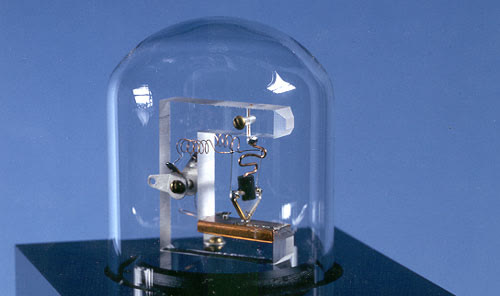
\includegraphics[width=0.42\linewidth]{images/book1/g9-first-transistor-replica.jpg}

{\small A replica of the first transistor of 1947, made for its fiftieth
anniversary: the triangle of plastic presses two gold contacts onto the
germanium below.}
\end{omfigure}

\section{Exercises}

\begin{exercise}[$\star$]\label{exo:g9:logic-gates:1}
A circuit is an \omterm{def:g9:logic-gates:not-and-or-xor}{OR gate} followed by a \omterm{def:g9:logic-gates:not-and-or-xor}{NOT gate}. What does it \omterm{def:g1:what-is-a-computer:input}{output} for
$a = 1$, $b = 0$? And for $a = 0$, $b = 0$?
\end{exercise}

\begin{exercise}[$\star$]\label{exo:g9:logic-gates:2}
Write the \omterm{def:g9:logic-gates:gate}{truth table} of XOR without looking, and say in words when its \omterm{def:g1:what-is-a-computer:input}{output}
is 1.
\end{exercise}

\begin{exercise}[$\star$]\label{exo:g9:logic-gates:3}
NAND is ``NOT AND''. Read the \omterm{def:g4:programs-and-operating-system:program}{program} below and write what it prints.

\omcode{code/grade-9/02-logic-gates/listings/nand_only.py}{1}{20}{NOT, AND and OR
from NAND alone.}\label{lst:g9:logic-gates:nand}
\end{exercise}

\begin{exercise}[$\star$]\label{exo:g9:logic-gates:4}
Write a \omterm{def:g7:functions:function}{function} \code{exactly_one(a, b, c)} that returns 1 when exactly one of
its three \omterm{def:g5:bits-and-bytes:bit}{bits} is 1.
\end{exercise}

\begin{exercise}[$\star\star$]\label{exo:g9:logic-gates:5}
This \omterm{def:g4:programs-and-operating-system:program}{program} should print the \omterm{def:g9:logic-gates:gate}{truth table} of AND. It prints one row only. Why?
Fix it.

\omcode{code/grade-9/02-logic-gates/exercises/table_bug.py}{1}{3}{A table with
missing rows.}\label{lst:g9:logic-gates:table-bug}
\end{exercise}

\begin{exercise}[$\star\star$]\label{exo:g9:logic-gates:6}
Someone draws a \omterm{def:g9:logic-gates:half-adder}{half adder} with an \omterm{def:g9:logic-gates:not-and-or-xor}{OR gate} for the sum \omterm{def:g5:bits-and-bytes:bit}{bit} instead of XOR.
Which \omterm{def:g1:what-is-a-computer:input}{input} gives a wrong answer, and what does the circuit then claim?
\end{exercise}

\begin{exercise}[$\star\star$]\label{exo:g9:logic-gates:7}
Write a \omterm{def:g4:programs-and-operating-system:program}{program} that prints the \omterm{def:g9:logic-gates:gate}{truth table} of
\code{(a OR b) AND (NOT c)}.
\end{exercise}

\begin{exercise}[$\star\star$]\label{exo:g9:logic-gates:8}
Write a \omterm{def:g7:functions:function}{function} \code{agree(f, g)} that tells whether two \omterm{def:g7:functions:function}{functions} of two
\omterm{def:g5:bits-and-bytes:bit}{bits} give the same \omterm{def:g1:what-is-a-computer:input}{output} on every \omterm{def:g1:what-is-a-computer:input}{input}.
\end{exercise}

\begin{exercise}[$\star\star$]\label{exo:g9:logic-gates:9}
How many rows does the \omterm{def:g9:logic-gates:gate}{truth table} of a circuit with 5 \omterm{def:g1:what-is-a-computer:input}{inputs} have? And with
10?
\end{exercise}

\begin{exercise}[$\star\star\star$]\label{exo:g9:logic-gates:10}
Prove with a \omterm{def:g9:logic-gates:gate}{truth table} that $a$ OR ($a$ AND $b$) $= a$ for all \omterm{def:g5:bits-and-bytes:bit}{bits} $a$ and
$b$. Then explain the rule in words.
\end{exercise}

\begin{exercise}[$\star\star\star$]\label{exo:g9:logic-gates:11}
A \omterm{def:g9:logic-gates:gate}{truth table} with two \omterm{def:g1:what-is-a-computer:input}{inputs} has four rows, each with an \omterm{def:g1:what-is-a-computer:input}{output} of 0 or 1.
How many different such tables are there? Show that each of them can be built
with NAND gates only.
\end{exercise}

\begin{exercise}[$\star\star\star$]\label{exo:g9:logic-gates:12}
Write a \omterm{def:g7:functions:function}{function} \code{add_two_bits(a1, a0, b1, b0)} that adds two numbers of
two \omterm{def:g5:bits-and-bytes:bit}{bits} each, $a_1a_0$ and $b_1b_0$, using \omterm{def:g9:logic-gates:half-adder}{half adders} and one \omterm{def:g9:logic-gates:not-and-or-xor}{OR gate}. It
returns three \omterm{def:g5:bits-and-bytes:bit}{bits}. Check it on all 16 \omterm{def:g1:what-is-a-computer:input}{inputs}.
\end{exercise}

\section{Problem: Three Judges and a Buzzer}

\begin{problem}[{Weekend problem --- three judges and a buzzer}]\label{pb:g9:logic-gates:1}
In a talent show, three judges each have a button. The buzzer sounds when at
least two of the three judges press.

\needspace{4\baselineskip}\medskip\noindent\textbf{Part I --- By hand.}
\begin{enumerate}
  \item Write the \omterm{def:g9:logic-gates:gate}{truth table}: 8 rows, with the \omterm{def:g1:what-is-a-computer:input}{inputs} $a$, $b$, $c$ (1 for a
    pressed button) and the \omterm{def:g1:what-is-a-computer:input}{output} (1 for the buzzer).
  \item In which rows does the buzzer sound? What do they have in common?
  \item Why do 8 rows cover every case?
\end{enumerate}

\needspace{4\baselineskip}\medskip\noindent\textbf{Part II --- Two circuits.}

\omcode{code/grade-9/02-logic-gates/listings/judges.py}{1}{29}{The rule, and two
circuits for it.}\label{lst:g9:logic-gates:judges}

\begin{enumerate}[resume]
  \item Explain the idea of \code{pairs}.
  \item Explain the idea of \code{majority}: what happens when $a$ and $b$
    agree, and when they do not?
  \item Run the \omterm{def:g4:programs-and-operating-system:program}{program}. Do the two circuits agree with the rule on all 8
    \omterm{def:g1:what-is-a-computer:input}{inputs}?
  \item Why does comparing them on 8 \omterm{def:g1:what-is-a-computer:input}{inputs} prove that they are right, and not
    just likely to be right?
\end{enumerate}

\needspace{4\baselineskip}\medskip\noindent\textbf{Part III --- Counting.}
\begin{enumerate}[resume]
  \item How many \omterm{def:g1:what-is-a-computer:input}{two-input} gates does \code{pairs} use? And
    \code{majority}?
  \item Draw the circuit of \code{pairs}.
  \item With five judges and ``at least three'', how many rows does the \omterm{def:g9:logic-gates:gate}{truth
    table} have?
  \item Which circuit would you build, and why?
  \item State the result.
\end{enumerate}
\end{problem}
